\documentclass[11pt]{article}

\usepackage{graphicx}
\usepackage{hyperref}
\usepackage{amsmath}
\usepackage{a4wide}
\usepackage{multirow}

\def\thetitle{Advanced Vision 2011/2012\\ Practical 3}
\def\theauthor{Steven Skelton (s0824321) and Wenqi Yao (s0838969)}

% TITLE PAGE
\title{\thetitle}
\author{\theauthor}
\date{}

\begin{document}

\maketitle
\thispagestyle{empty}

\section{Introduction}

In this assignment, we were tasked with augmenting a sequence of images, via homographic transfer of a given background image, and a sequence of images from a separate video.

\section{Algorithms}
\subsection{Finding the Background}
The points in the trapezoid are found manually and hard-coded into the background-finding algorithm. \\

To find the points of interest (within the back wall), the equations of the lines between neighbouring corners are found. Naive interpolation is used to find pixels on the lines. \\

Each row of pixels within the bounding rectangle are scanned to find the left-most and right-most pixels in each line. All pixels between these two pixels (inclusive) are marked on a indicator matrix of size \emph{480 x 640}. \\

To find the foreground, the z-values for each pixel are averaged over the first 7 frames (before the man walks in). In each frame, the foreground is then given by every pixel that is at least a threshold value in front of its mean value. \\

At the top of the image, the pixels are further away and have a smaller variance. Many pixels remain as background pixels throughout, and hence many of them are cast as ``foreground" pixels over different frames. Hence, the threshold value is set at 0.1. \\

At the bottom of the image, the pixels are nearer, with a large variance. Most of the pixels will be covered by the walking man's legs in at least one frame. Using 0.1 as the threshold value hence causes incorrect classification of the man's trousers as the background (as seen in Figure \ref{failbg}). Instead, the threshold is set to the standard deviation of each pixel over all frames. \\

The classified background pixels are then masked with the indicator matrix.

\begin{figure}
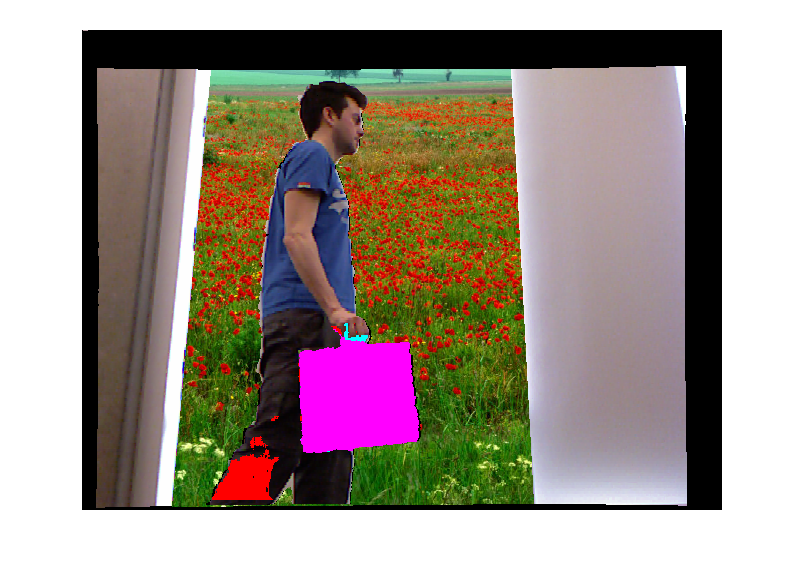
\includegraphics[width=\textwidth]{floatingman}
\caption{Using 0.1 as the threshold causes incorrect classification of lower pixels.}
\label{failbg}
\end{figure}

\subsection{Image Transfer}

To transfer the given image of the field onto the background pixels, the given code for homographic transfer \emph{(esthomog.m)} is used. Due to the crude nature of the interpolation between corners, some of the pixels in the background area map to points just outside the boundaries of the field image. These pixels are capped to the boundary of the field image. 

\subsection{Finding the Plane}

Various techniques were used in attempts to find the plane.

\subsubsection{Pruning the Search Space}

\subsubsection{RANSAC}
A RANSAC plane-finding algorithm was tried. In each iteration, 3 random points were picked and a plane was fit to them. If the number of points within the search space that fit the plane (to a given threshold, around 0.005) was between 10000 and 15000, the plane was considered as a candidate plane. After 100 iterations, the candidate plane with the smallest sum error between itself and the points that lay on it was returned. \\

The problem with this method was that it was extremely slow, and often returned planes that did not 

\subsection{Estimating the corners of the rectangle}

\section{Results}


\section{Conclusion}

\end{document}
